\chapter {Introducción}
\label{sec:intro}

\section {Planteamiento del problema}

\begin{flushright}
\begin{minipage}[b][4cm][t]{11cm}
\begin{flushright}
{\small \emph{No hay alternativa a la transformación digital.}} \vspace{-1pt} \\
{\small \emph{Las compañías visionarias crearán nuevas opciones}} \vspace{-1pt} \\
{\small \emph{estratégicas para sí mismas.}} \vspace{-1pt} \\
{\small \emph{Aquellas que no se adapten, fracasarán.}} \vspace{1mm}\\
{\footnotesize Jeff Bezos,} \vspace{-1.5pt} \\
{\footnotesize fundador de Amazon.\phantom{l}}
\end{flushright}
\end{minipage}
\end{flushright}

En la actualidad,  la transformación digital se ha convertido en una necesidad acuciante para todas las organizaciones \cite{DigitalBT}. Este mensaje puede ser escuchado alta y claramente en cada discusión o artículo donde se intenta aclarar qué pueden hacer las empresas para seguir siendo relevantes en un mundo cada vez más digitalizado y globalizado. 

Como suele ocurrir, son las pequeñas y medianas empresas las que más dificultades experimentan para enfrentar nuevos retos. Mientras que las grandes compañías ya han adquirido tecnología y contratado personal especializado para tratar con esta problemática, algunos pequeños negocios ni siquiera son conscientes de la magnitud del cambio que les espera. Sin embargo, aunque haya empresas mejor preparadas que otras, todas deben alcanzar el mismo destino y para ello cada una debe encontrar su propio camino.

En 2018 el ITRE encargó un estudio para obtener información sobre cómo la Unión Europea puede aprovechar la oportunidad que plantea el uso de la inteligencia artificial. Uno de los puntos que trata esta investigación es la aceptación de la IA en las empresas europeas. En él se refleja que tan sólo un 20\% de las organizaciones usan esta tecnología actualmente. El porcentaje de pymes es mucho más bajo, únicamente supone un 5\% sobre el total \cite{EuropeAI}. A continuación, se muestra un gráfico donde se recoge el porcentaje de empresas que hacen uso de soluciones o servicios de IA:

\begin{figure}[htbp]
	\begin{center}
		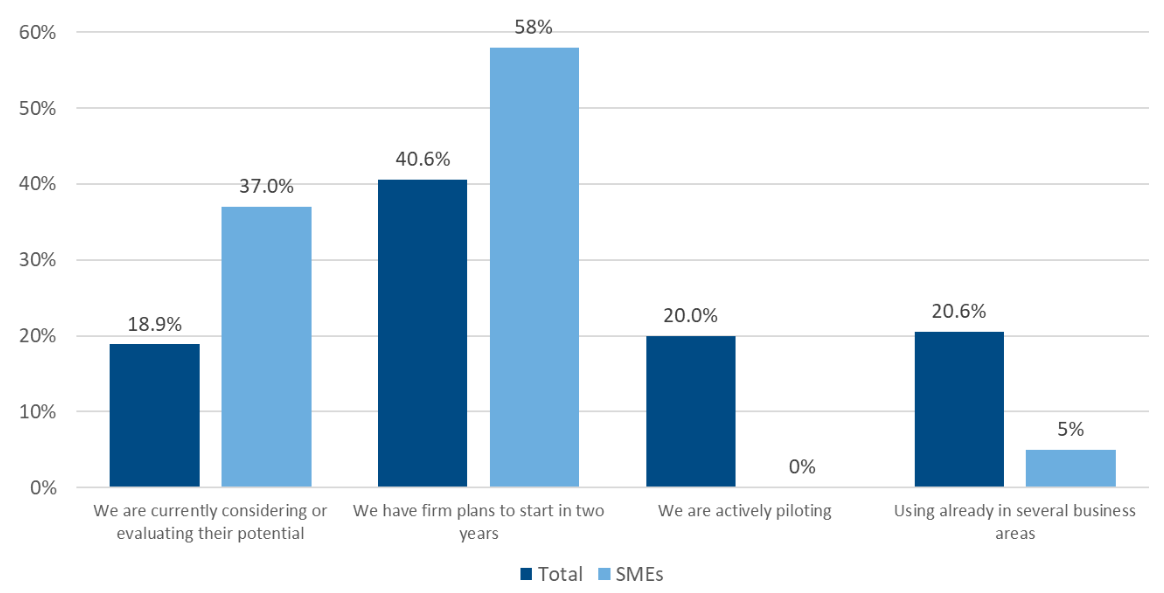
\includegraphics[width = 1\textwidth]{Figuras/AIUse.PNG}
	\end{center}
	\caption{\label{fig:AIBarriers} Uso de servicios/soluciones de IA en Europa (Total de empresas frente a pymes). Fuente: Encuesta de soluciones cognitivas/IA de Europa occidental realizada por IDC, junio 2018 (n = 350).}
\end{figure}

\newpage

Las pymes pueden encontrar una magnífica solución para cumplir con sus necesidades en el Cloud Computing. Los servicios en la nube que ofrecen grandes proveedores como Google, Microsoft o Amazon ponen al alcance de estas empresas la tecnología que antes sólo se podían permitir las grandes organizaciones. Además, al ser recursos completamente gestionados por las empresas proveedoras, las organizaciones pueden centrarse más en su negocio y abstraerse de la infraestructura o la disponibilidad de su sistema. 

La integración de herramientas de IA mediante computación en la nube, en un negocio electrónico, puede ayudar a conseguir los objetivos que persigue la transformación digital. 

La transformación digital lidera un enfoque de negocio centrado en el cliente que busca comprender correctamente los cambios en los comportamientos de los clientes y cómo hacerles llegar los servicios adecuadamente. Se trata además de digitalizar los procesos de negocio y los canales de comunicación, mejorando de esta forma la experiencia de cliente. 

Para entender mejor a los clientes puede resultar muy útil para las organizaciones analizar los sentimientos de los comentarios que éstos publican. En este proyecto se pretende integrar una herramienta que permita llevar a cabo esta acción en una tienda electrónica.

También es muy importante que la empresa garantice una buena experiencia al cliente cuando haga uso de sus servicios. Con esta idea en mente, se quiere además implementar una interfaz conversacional que ayude a ofrecer un servicio más personalizado al consumidor y facilite la navegación por el sitio web a usuarios menos familiarizados con esta plataforma. Este servicio estará disponible en todo momento, aliviando la carga de trabajo de los empleados de atención al cliente. No se debe olvidar que este departamento es la cara visible de la organización e influye directamente sobre la satisfacción de los clientes.

Por último, se persigue asegurar la disponibilidad de estas herramientas y de la propia tienda electrónica haciendo uso de la tecnología de contenerización en la nube.

\section {Objetivos del proyecto}

Este trabajo tiene por objetivo general comprobar el funcionamiento de la Inteligencia Artificial como herramienta de marketing digital en una web. 

Con este fin se creará un portal de comercio electrónico donde se integrarán un servicio de análisis de sentimientos y un bot conversacional. Asimismo, la solución será desplegada en la nube utilizando contenedores.

Los objetivos específicos de este proyecto son:
\begin{itemize}
    \item Aprender a usar los servicios de la nube relacionados con IA y machine learning.
    \item Aprender a diseñar una aplicación con una arquitectura basada en microservicios. 
    \item Aprender a implementar una arquitectura cliente-servidor.
    \item Aprender a desplegar una aplicación en la nube. 
    \item Aprender a utilizar contenedores para el despliegue y desarrollo de una aplicación.
    \item Demostrar la utilidad y escalabilidad de los sistemas basados en cloud.
\end{itemize}

\section {Organización del trabajo}

El trabajo está dividido en siete capítulos que guiarán al lector a través de todo el proceso de desarrollo de la solución propuesta. En este primer capítulo se ofrece una visión general del problema que se pretende resolver y se plantean los objetivos a alcanzar.

\newpage
 
En el segundo capítulo se persigue contextualizar el trabajo describiendo las diferentes áreas de estudio relacionadas con el mismo. Se divide en cinco secciones. En la primera sección se tratará la situación actual de la computación en la nube y se presentarán sus principales características, así como los modelos de servicio más habituales. La segunda sección está destinada a definir el concepto de comercio electrónico y sus principales categorías. Además, se discutirá sobre el presente y futuro de este campo. En la tercera sección, se expondrán los beneficios de aunar computación en la nube y comercio electrónico.

La cuarta sección describe cómo la inteligencia artificial ha dejado de ser una herramienta al servicio de unas pocas organizaciones para convertirse en un recurso accesible a la mayoría de empresas gracias los servicios de computación en la nube.

La quinta sección se ocupa del análisis de sentimientos, se intentará aclarar en qué consiste y  cómo puede ayudar a las empresas. También se presentarán otras aplicaciones más allá de los usos comerciales. Por último, se establecerá una comparación entre algunos de los servicios cloud de análisis de sentimientos más importantes. De forma similar, en la sexta sección se hablará sobre el concepto de interfaz conversacional, ofreciendo una visión de la evolución que ha sufrido esta tecnología hasta la fecha y tratando algunas de las ventajas de su aplicación al comercio electrónico. Se finalizará comparando diferentes herramientas cloud que permiten desarrollar una interfaz de este tipo.

En el tercer capítulo se definirán las etapas en las que de ha dividido el proyecto, ofreciendo una breve explicación sobre cada una de ellas. Igualmente, se comparará la estimación de horas planteada antes de comenzar con el proyecto y los tiempos reales invertidos.

En el cuarto capítulo se propone la solución escogida. Está compuesto por cinco secciones. En la primera sección es donde se realiza un análisis de esta solución, pero sin tener en cuenta aspectos de la implementación. Simplemente, se trata de explicar la idea que se pretende desarrollar y cómo se planea llevarla a cabo. Dicha solución estará formada por tres elementos principales: página web, análisis de sentimientos e interfaz conversacional. En la segunda sección se detallarán los casos de uso del sistema, incluyendo un diagrama de casos de uso, la especificación de los actores y la de cada uno de los casos de uso. La tercera y cuarta sección están incluirán un análisis de requisitos, funcionales y no funcionales, respectivamente.
Para finalizar este capítulo, en la cuarta sección se realizará un estudio económico del proyecto, detallando las tarifas de cada uno de los servicios en la nube y los costes directos e indirectos en los que incurre la realización del proyecto.

En el quinto capítulo se enumerarán las diferentes herramientas utilizadas para el desarrollo del proyecto y se dará información sobre su utilidad. Se ha obviado mencionar aquellas herramientas relacionadas con la realización de la memoria. 
\newpage
El capítulo seis es el eje central del trabajo. Se divide en tres secciones. En la primera sección se explicará la arquitectura del sistema desarrollado. En la segunda sección se realizará un descripción pormenorizada del proceso de implementación para la página web, la herramienta de análisis de sentimientos y la interfaz conversacional. Asimismo, la tercera sección se ocupa de realizar una explicación similar destinada a exponer como desplegar estos componentes en la nube, para lo que se hará uso de contenedores. 

Por último, en el capítulo siete se valorarán los resultados obtenidos tras haber completado el proyecto. Este capítulo consta de dos secciones. En la primera sección se reflexionará sobre los conocimientos adquiridos por el alumno. En la segunda sección se plantearán posibles líneas de trabajo futuro con las que poder continuar mejorando el proyecto.